\documentclass[crop=false, class=memoir]{standalone}

\usepackage[utf8]{inputenc}%Nødvendig for danske bogstaver
\usepackage[danish]{babel}%Sørger for at ting LaTeX gør automatisk er på dansk
\usepackage{csquotes}
\usepackage{geometry}%Til opsætning af siden
\geometry{lmargin = 2.5cm,rmargin = 2.5cm}%sætter begge magner
\usepackage{lipsum}%Fyldtekst, til brug under test af layoutet
\usepackage{float}
\usepackage{graphicx}%Tillader grafik
\usepackage{epstopdf}%Tillader eps filer
\usepackage{marginnote}% Noter i margen
\interfootnotelinepenalty=10000 %undgår at fodnoter bliver spilittet op.
\usepackage[sorting=none]{biblatex}
\addbibresource{litteratur.bib}
\usepackage[hidelinks]{hyperref}%Tillader links
\usepackage{subcaption} % Tillader underfigurer
\usepackage[font={small,sl}]{caption}	% Caption med skrå tekst ikke kursiv

\usepackage{xcolor} %Bruges til farver
\usepackage{forloop} %Bruges til nemmere for loops

\newcounter{opgave}[chapter] %Definerer opgavenumrene og hvornår de nulstilles
\renewcommand{\theopgave}{\thechapter.\arabic{opgave}} %Definerer udseende af opgavenummereringen
\newcounter{delopgave}[opgave] %Definerer delopgavenumrene
\newcounter{lvl} %Definerer en "variabel" til senere brug

\definecolor{markerColor}{rgb}{0.0745098039, 0.262745098, 0.584313725} %Definerer farven af markøren
\newcommand{\markerSymbol}{\ensuremath{\bullet}} %Definerer tegnet for markøren
\newlength{\markerLength} %Definerer en ny længde
\settowidth{\markerLength}{\markerSymbol} %Sætter den nye længde til bredden af markøren

\newenvironment{opgave}[2][0]{%Definerer det nye enviroment, hvor sværhedsgraden er den første parameter med en default på 0
\newcommand{\opg}{\refstepcounter{delopgave}\par\vspace{0.1cm}\noindent\textbf{\thedelopgave)\space}}%Definerer kommando til delopgave
\refstepcounter{opgave}%Forøger opgavenummer med 1 og gør den mulig at referere til
\setcounter{lvl}{#1}%Sætter "variablen" lvl lig med angivelsen af sværhedsgraden
\noindent\hspace*{-0.75em}\hspace*{-\value{lvl}\markerLength}\forloop{lvl}{0}{\value{lvl}<#1}{{\color{markerColor}\markerSymbol}}\hspace*{0.75em}%Sætter et antal af markører svarende til sværhedsgraden
\textbf{Opgave \theopgave : #2}\newline\nopagebreak\ignorespaces}{\bigskip} %Angiver udseende af titlen på opgaverne samt mellemrummet mellem opgaver



\usepackage{mathtools}%Værktøjer til at skrive ligninger
\renewcommand{\phi}{\varphi}%Vi bruger varphi
\renewcommand{\epsilon}{\varepsilon}%Vi bruger varepsilon
\usepackage{physics}%En samling matematikmakroer til brug i fysiske ligninger
\usepackage{braket}%Simplere kommandoer til bra-ket-notation
\usepackage{siunitx}%Pakke der håndterer SI enheder godt
\DeclareSIUnit\clight{\text{\ensuremath{c}}} % Lysets fart i vakuum som c og ikke c_0
\usepackage{chemmacros}
\usechemmodule{isotopes}
\usepackage{tikz}
\usepackage[danish]{cleveref}
\usepackage{nicefrac}
% \renewcommand{\ref}[1]{\cref{#1}}
\creflabelformat{equation}{#2(#1)#3}
\crefrangelabelformat{equation}{#3(#1)#4 to #5(#2)#6}
\crefname{equation}{ligning}{ligningerne}
\Crefname{equation}{Ligning}{Ligningerne}
\crefname{section}{afsnit}{afsnitene}
\Crefname{section}{Afsnit}{Afsnitene}
\crefname{figure}{figur}{figurene}
\Crefname{figure}{Figur}{Figurene}
\crefname{table}{tabel}{tabellerne}
\Crefname{table}{Tabel}{Tabellerne}
\crefname{opgave}{opgave}{opgaverne}
\Crefname{opgave}{Opgave}{Opgaverne}
\crefname{delopgave}{delopgave}{delopgaverne}
\Crefname{delopgave}{Delopgave}{Delopgaverne}

\newcommand{\eqbox}[1]{\begin{empheq}[box=\fbox]{align}
	\begin{split}
	#1
	\end{split}
\end{empheq}}

\newcommand{\kb}{\ensuremath{k_\textsc{b}}}

\DeclareSIUnit{\parsec}{pc}
\DeclareSIUnit{\lightyear}{ly}
\DeclareSIUnit{\astronomicalunit}{AU}
\DeclareSIUnit{\year}{yr}
\DeclareSIUnit{\solarmass}{M_\odot}
\DeclareSIUnit{\solarradius}{R_\odot}
\DeclareSIUnit{\solarluminosity}{L_\odot}
\DeclareSIUnit{\solartemperature}{T_\odot}
\DeclareSIUnit{\earthmass}{M_\oplus}
\DeclareSIUnit{\earthradius}{R_\oplus}
\DeclareSIUnit{\jupitermass}{M_J}

% Infobokse og lignende
% http://mirrors.dotsrc.org/ctan/graphics/awesomebox/awesomebox.pdf
% \usepackage{awesomebox}


% Egen infobokse (virker kun med begrænsede symboler)

\usepackage[framemethod=tikz]{mdframed}
\usetikzlibrary{calc}
\usepackage{kantlipsum}

\usepackage[tikz]{bclogo}

\tikzset{
    % lampsymbol/.style={scale=2,overlay}
    % lampsymbol/.pic={\centering\tikz[scale=5]\node[scale=10,rotate=30]{\bclampe}}.style={scale=2,overlay}
    infosymbol/.style={scale=2,overlay}
}

\newmdenv[
    hidealllines=true,
    nobreak,
    middlelinewidth=.8pt,
    backgroundcolor=blue!10,
    frametitlefont=\bfseries,
    leftmargin=.3cm, rightmargin=.3cm, innerleftmargin=2cm,
    roundcorner=5pt,
    % skipabove=\topsep,skipbelow=\topsep,
    singleextra={\path let \p1=(P), \p2=(O) in ($(\x2,0)+0.92*(1.1,\y1)$) node[infosymbol] {\bcinfo};},
    % singleextra={\path let \p1=(P), \p2=(O) in ($(\x2,0)+0.5*(2,\y1)$) node[infosymbol] {\bcinfo};},
]{info}

% Skal bruges som
% \begin{info}[frametitle={Titel}]
%     Tekst
% \end{info}
% Infobokse og lignende
% http://mirrors.dotsrc.org/ctan/graphics/awesomebox/awesomebox.pdf
% \usepackage{awesomebox}


% Egen infobokse (virker kun med begrænsede symboler)

\usepackage[framemethod=tikz]{mdframed}
\usetikzlibrary{calc}
\usepackage{kantlipsum}

\usepackage[tikz]{bclogo}

\tikzset{
    % lampsymbol/.style={scale=2,overlay}
    % lampsymbol/.pic={\centering\tikz[scale=5]\node[scale=10,rotate=30]{\bclampe}}.style={scale=2,overlay}
    infosymbol/.style={scale=2,overlay}
}

\newmdenv[
    hidealllines=true,
    nobreak,
    middlelinewidth=.8pt,
    backgroundcolor=blue!10,
    frametitlefont=\bfseries,
    leftmargin=.3cm, rightmargin=.3cm, innerleftmargin=2cm,
    roundcorner=5pt,
    % skipabove=\topsep,skipbelow=\topsep,
    singleextra={\path let \p1=(P), \p2=(O) in ($(\x2,0)+0.92*(1.1,\y1)$) node[infosymbol] {\bcinfo};},
    % singleextra={\path let \p1=(P), \p2=(O) in ($(\x2,0)+0.5*(2,\y1)$) node[infosymbol] {\bcinfo};},
]{info}

% Skal bruges som
% \begin{info}[frametitle={Titel}]
%     Tekst
% \end{info}

\begin{document}

\chapter{Laserfysik} \label{chap:laser}
\section{Introduktion}
Valgemnet om ekperimentel laserfysik handler om at bygge et optisk interferometer. Dette kapitel af kompendiet gennemgår den teori, der skal til, for at forstå, hvordan inteferometret fysisk virker.

I første omgang skal vi bruge en teoretisk beskrivelse af lyset fra laseren, men hvad er lys egenligt? Du har sikkert hørt at lys både er bølger (i det elektromagnetiske felt) og partikler (fotoner), afhængigt af hvordan man observerer det. Det er også rigtigt, men til at beskrive vores optiske interferometer, er det bølgebeskrivelsen af lys, vi skal bruge.

\section{Lys som bølger}
Lys kan beskrives som bølger. Men for at have en bølge, skal vi også have et medie den bølge svinger i, for eksempel er bølgerne på havet svingninger i vandoverfladen. Så hvilket medie er lys svingninger i? Fordi lys kan rejse igennem det tomme rum, troede man i lang tid, at det var bølger i et medie, man kaldte ``æteren''. I slutningen af 1800 tallet byggede Albert Michelson og Edward Morley dog et interferometer, meget lig det vi skal bygge i dette valgemne, og med det kunne de tage målinger, der modviste hypotensen om æteren. Vores nuværende forståelse er i stedet, at lyset er svingninger direkte i de elektriske og magnetiske felter. 

Alle elektriske og magnetiske felter opfylder Maxwells ligninger, og det samme gælder for lys. Ud fra Maxwells ligninger kan man også finde mange af de basale egenskaber for lys, som vi skal bruge i vores eksperiment:

\begin{itemize}
    \item Svingningen af det elektriske og magnetiske felt er sinusbølger. Det gælder både i tid og i rum.
    \item Lys er transverse bølger. Det vil sige, at svingningen i de elektriske og magnetiske felt er vinkelret på udbreddelsesretningen af lyset. Det er illustreret i figur \ref{laser:fig:EMBolge}, hvor lyser bevæger sig i $x$-retningen, mens svingningen i det elektriske og magnetiske felt er vinkeltrette på denne retning, og på hinanden. Af den grund behøver vi ikke tænke over hvilken retningen det magnetiske felt svinger i, så længe vi beskriver svingningen af det elektriske felt.
    \item Polariseringen af lys beskriver, hvilken retning det elektriske felt svinger i. Forestil dig, at en stråle af lys fra en laser bevæger sig parallelt med et bord. Hvis det elektriske felt svinger op og ned, kalder vi det vertikalt polariseret. Hvis det svinger til fra side til side parallelt med bordet, kalder vi det horisontalt polariseret.
    \item Lys bevæger sig med lysets hastighed i vakuum, altså $c = \SI{299792458}{\metre\per\second}$, uanset af hvilken frekvens  svingningerne har. I et andet materiale end vakuum, bevæger det sig i stedet med en hastighed, der afhænger af materialet. Den beskriver man typisk ved hjælp af lysets brydningsindeks i materialet, $n$. Dermed bliver lysets hastighed i materialet: $c_\textup{mat} = c/n$. Dog er lufts brydningsindekset meget tæt på 1 ($n_\textup{luft} = \num{1.000293}$), så i vores beskrivelse bruger vi bare lysets hastighed i vakuum.
\end{itemize}

\section{Matematisk beskrivelse af lys} \label{laser:sec:mat_lys}
Ud fra disse egenskaber for lys vil vi nu opstille en matematisk beskrivelse vi kan bruge til analyser. For det første ved vi, at hvis vi beskriver det elektriske felt, så er der ikke mere information at hente, i at beskrive det magnetiske felt -- kender vi det elektriske felt, kan det magnetiske felt beregnes. Derfor vil vi beskrive, hvordan det elektriske felt svinger i tid og rum. Vi beskriver derfor det elektriske felt med en funktion, der afhænger af tiden, $t$, og positionen, $x$. Her er $x$ en position langs udbredelsesretningen af lyset, som på \cref{laser:fig:EMBolge}.

\begin{figure}
    \centering
    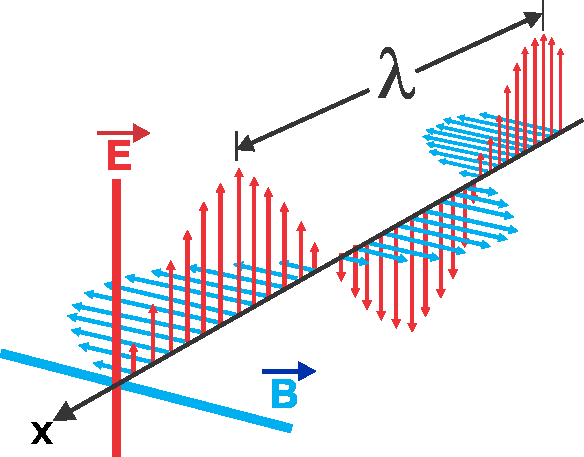
\includegraphics[width=0.42\linewidth]{Laserfysik/billeder/EMBolge.pdf}
    \caption{Det elektriske og magnetiske felt i en lysbølge henholdsvis markeret med symbolerne $\va{E}$ og $\va{B}$. Derudover er bølgelængden $\lambda$ indtegnet.}
    \label{laser:fig:EMBolge}
\end{figure}

Vi ved, at vores lys skal svinge i både tid og rum som en sinusbølge. Hvis vi siger, at amplituden af bølgen er $E_0$, kan vi dermed skrive den som:
%
\begin{align}\label{laser:eq:simpeltEFelt}
    E(t, x) = E_0  \cdot \sin(\omega\cdot t - k\cdot x).
\end{align}
%
\emph{Vinkelfrekvesen} af lyset, $\omega$, kan vi relatere til bølgelængden. I \cref{laser:fig:EMBolge} er det tydeligt, at lyset bevæger sig én \emph{bølgelængde}, $\lambda$, for hver gang det svinger fra bølgetop til bølgedal og tilbage til en bølgetop igen. Det sker med en frekvens\footnote{Faktoren af $2\cdot\pi$ kommer her fra, at frekvensen $\omega$ ikke er en ren frekvens, men en vinkelfrekvens, der måles i radianer per sekund. Da der er $2\cdot\pi$ radianer rundt i en cirkel, skal vi dividere $\omega$ med $2\cdot\pi$, for at finde frekvensen af svingningen.} på $\omega/(2\cdot\pi)$. Hvis vi ganger længden af bølgen, $\lambda$, med hvor mange bølger, der svinger per tid, finder vi hastigheden af bølgen, der for lys må være lysets hastighed, $c$. Dermed kan vi udlede en sammenhæng mellem vinkelfrekvensen og bølgelængden af lyset:
%
\begin{align}
    \lambda \cdot \frac{\omega}{2\cdot\pi} = c \qquad \implies \qquad \omega = \frac{2\cdot\pi\cdot c}{\lambda}.
\end{align}
%
\emph{Bølgetallet}, $k$, beskriver hvor hurtigt bølgen svinger, når vi kigger på den i den rumlige dimension langs bevægelsesretningen\footnote{At der står $-k\cdot x$ i \cref{laser:eq:simpeltEFelt} er ikke en fejl, men er nødvendigt for at lysbølgen bevæger i den positive $x$-retning. Hvis vi går lidt fremad langs bølgen, kommer vi lidt foran, hvordan den svinger i tid, altså svarer det til at gå tilbage i tiden. Dermed skal svingningen i position have modsat effekt af svingningen i tid, hvilket svarer til det negative fortegn.}. Hvis vi bevæger os en bølgelængde langs lysbølgen, skal den gå fra bølgetop til bølgedal og tilbage til bølgetop igen. Det svarer til at $k\cdot \lambda$ skal bidrage med en hel svingning af bølgen, og skal dermed være lig $2\cdot \pi$:
%
\begin{align}
    k \cdot \lambda = 2\cdot \pi \qquad \implies \qquad k = \frac{2\cdot \pi}{\lambda}.
\end{align}
%
Dermed kan svingningen af vores elektriske felt, der også kaldes E-feltet, altså skrives som:
%
\begin{align}
    E(t, x) = E_0 \cdot \sin\left(\frac{2\cdot\pi\cdot c}{\lambda} \cdot t - \frac{2\cdot\pi}{\lambda} \cdot x\right).  
\end{align}
%
Endeligt ved vi, at lyset svinger i en retning der er vinkelret på udbredelsesretnignen af lyset (som vi her har valgt til at være $x$). For at beskrive dette i vores formel, beskriver vi det elektriske felt som en vektor. Her introducerer vi polarisationsretningen som vektoren $\va{e}$, der kaldes \emph{polarisationsvektoren}. Den har altid en længde på 1 (det er en enhedsvektor), og en retning der peger vinkelret på bevægelsesretningen af lyset.
%
\begin{align}\label{laser:eq:EFeltFinal}
    \va{E}(t, x) = E_0 \cdot \va{e} \cdot \sin\left(\frac{2\cdot\pi\cdot c}{\lambda} \cdot t - \frac{2\cdot\pi}{\lambda} \cdot x\right)
\end{align}
%
Her har vi vores endelige formel for vores elektromagnetiske lysbølge. 

\section{Lysets intensitet} \label{laser:sec:intensitet}
%
Ofte er det praktisk at arbejde med energien, der i lyset, og til det formål bruges lysets \emph{intensitet}, $I$. Intensiteten er defineret som \emph{mængden af energi der transporteres af lyset per areal, per tid}. Sagt på en anden måde er det lysets effekt per areal. Intensiteten er proportional til længden af E-feltsvektoren i anden:
%
\begin{align}
    I = \frac{c\cdot n \cdot \epsilon_0}{2} \cdot | \va{E}(t, x) |^2.
\end{align}
%
Når vi udregner intensiteten lyserts elektriske felt, \cref{laser:eq:EFeltFinal}, er det godt at huske at længden af polarisationsvektoren er 1, $|\va{e}|^2 = 1$:
%
\begin{align}
    I &= \frac{c \cdot n \cdot \epsilon_0}{2} \cdot E_0^2 \cdot |\va{e}|^2 \cdot \sin^2 \left(\frac{2\cdot\pi\cdot c}{\lambda} \cdot t - \frac{2\cdot\pi}{\lambda} \cdot x\right) \\
    &= \frac{c \cdot n \cdot \epsilon_0}{2} \cdot E_0^2 \cdot \sin^2 \left(\frac{2\cdot\pi\cdot c}{\lambda} \cdot t - \frac{2\cdot\pi}{\lambda} \cdot x\right).
\end{align}
%
For en bestemt position $x$ ser vi, at intensiteten af lyset svinger i tid, mellem 0 og 1. Dog er svingningen af lys meget hurtig\footnote{F.eks. har det røde lys fra en Helium-Neon-laser en bølgelængde på cirka \SI{633}{\nano\meter}, så frekvensen af lyset fra den bliver: $\omega_\textup{HeNe} = 2\cdot \pi \cdot c/(\SI{633}{\nano\meter}) = \SI{2.976e15}{\radian\per\second} = \SI{4.74e14}{\hertz}$, altså svinger lyset frem og tilbage ca. 474 billioner gange i sekundet!}, så ofte bruger vi den gennemsnitlige intensitet i tid, fordi det er det, vores øjne og detektorer kan se alligevel.  Heldigvis er gennemsnittet af $\sin^2(\omega\cdot t)$ altid $1/2$, uanset hvad $\omega$ er. Altså er den gennemsnitlige (engelsk: average) intensitet
%
\begin{align}
    I_\textup{avg} = \frac{c\cdot n \cdot \epsilon_0}{2} E_0^2,
\end{align}
%
hvilket er rimelig pænt. 

\section{Analyse af Michelson interferometer}
%
\begin{figure}
    \centering
    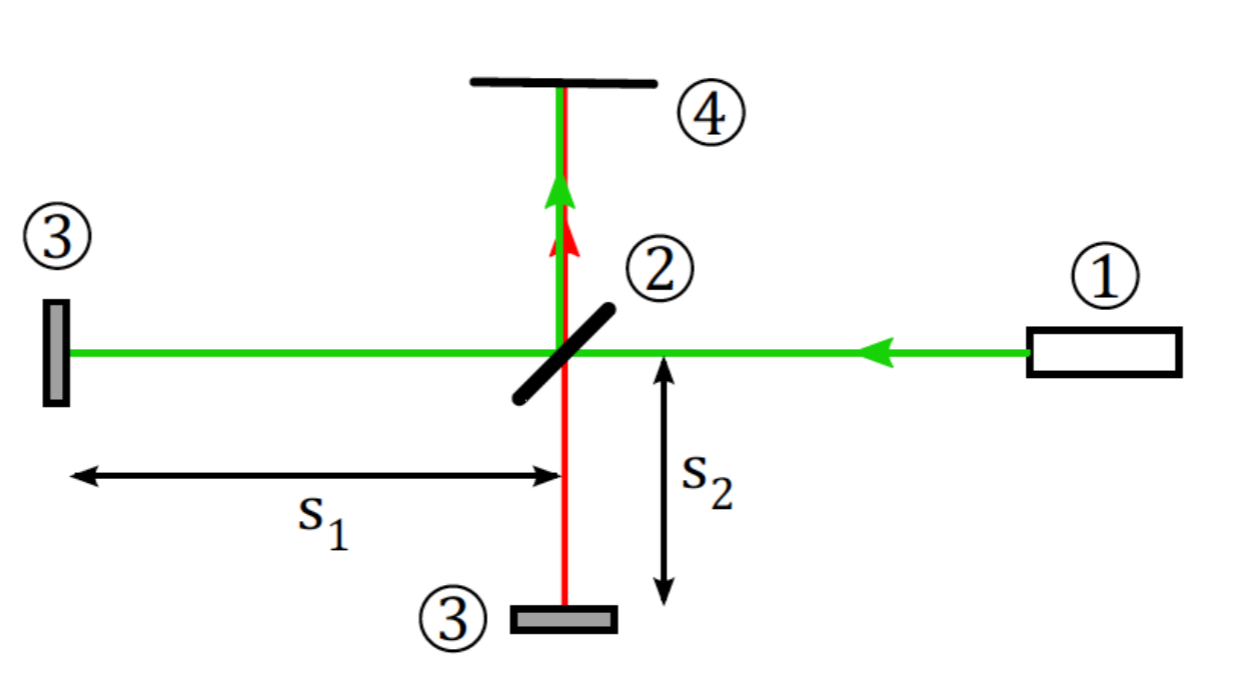
\includegraphics[width=0.5\linewidth]{Laserfysik/billeder/Setup.PNG}
    \caption{Opstilling af et Michelson interferometer. På tegningen er der vist: 1: En laser, der skyder en laserstråle ud. 2: En beamsplitter, der splitter denne laserstråle i to stråler. 3: 2 spejle, der reflekterer de to laserstråler tilbage på beamsplitteren. 4: En skærm, hvor vi kan se interferensmønsteret. De to veje, som laserstrålerne tager efter beamsplitteren, har forskellig vejlængde, som her er kaldt $s_1$ og $s_2$.}
    \label{fig:michelsonInterferometer}
\end{figure}
%
Opstillingen af et Michelson interferometer kan ses i \cref{fig:michelsonInterferometer}. Hele pointen med opstillingen er, at en lysstråle deles op i 2 veje, rejser 2 forskellige vejlængder, for derefter at blive kombinerede igen. De to veje imellem beamsplitteren og spejlene kaldes også for interferometrets arme.

Først ser vi på hvor meget lys, der kommer ud af hver beamsplitter, altså, hvilken værdi $E_0$ skal have i hver af de to stråler. Det gør vi ud fra kravet om, at der skal være energibevarelse. For at energien er bevaret, skal intensiteten af lyset, der jo er energi per tid, per areal, være bevaret. Derfor kommer vi frem til at intensiteten i hver stråle, er halvedelen af den oprindelige stråle:
%
\begin{align}
    I_1 = I_2 &= \frac{I}{2} \\
    \implies \frac{c\cdot n \cdot \epsilon_0}{2} E_{0,1}^2 &= \frac{(c\cdot n \cdot \epsilon_0/2)\cdot E_{0}^2}{2} \\ 
    \implies E_{0, 1}^2 &= \frac{E_0^2}{2} \\
    \implies E_{0, 1} &= \frac{E_0}{\sqrt{2}}.
\end{align}
%
Den oprindelige E-feltsamplitude skal derfor ganges med en faktor $1/\sqrt{2}$, for at få amplituden af hver stråle efter beamsplitteren. Dog passerer hver stråle gennem beamsplitteren en gang mere på vej tilbage, så derfor skal vi dividere den endelige E-feltsamplitude af hver stråle med $2$ i stedet for $\sqrt{2}$, for at få den amplitude som når detektoren:
%
\begin{align}
    \va{E}_{1}(t, x) = \frac{E_0}{2} \cdot \va{e} \cdot \sin\left(\frac{2\cdot\pi\cdot c}{\lambda} \cdot t - \frac{2\cdot\pi}{\lambda} \cdot x\right).
\end{align}
%
Lad os prøve at måle, hvor langt hver lyststråle rejser, efter de bliver splittet ved beamsplitteren \Circled{2}. 
%
\begin{itemize}
    \item Stråle 1 passerer lige igennem beamsplitteren, og rejser først en afstand på $s_1$ hen til sit spejl, så en afstand $s_1$ tilbage til beamsplitteren. Her reflekteres halvdelen af den og rejser en afstand $l$ hen til skærmen.
    \item Stråle 2 bliver reflekteret af beamsplitteren, rejser en afstand $s_2$ frem og tilbage fra sit spejl, hvorefter halvdelen passerer gennem beamsplitteren, som så rejser en afstand $l$ hen til skærmen.
\end{itemize}
%
Dermed bliver vejlængderne:
%
\begin{align}\label{laser:eq:vejlangde}
    x_1 &= 2\cdot s1 + l,\\
    x_2 &= 2\cdot s2 + l.
\end{align}
%
Vi skriver det samlede E-felt for de to lysstråler op ved skærmen \Circled{4} og bruger at begge stråler har samme polarisering:
%
\begin{align}
    \va{E}_{tot}(t, x) &= \va{E}_1(t, x_1) + \va{E}_2(t, x_2)\\
    &= \frac{E_{0}}{2} \cdot \va{e_1} \cdot \sin\left(\frac{2\cdot\pi\cdot c}{\lambda} \cdot t - \frac{2\cdot\pi}{\lambda} \cdot x\right)  + \frac{E_0}{2} \cdot \va{e_2} \cdot \sin\left(\frac{2\cdot\pi\cdot c}{\lambda} \cdot t - \frac{2\cdot\pi}{\lambda} \cdot x\right)\\
    &= \frac{E_0}{2} \cdot \va{e_1} \cdot \left(   
    \sin\left(\frac{2\cdot\pi\cdot c}{\lambda} \cdot t - \frac{2\cdot\pi}{\lambda} \cdot x_1\right)
    + \sin\left(\frac{2\cdot\pi\cdot c}{\lambda} \cdot t - \frac{2\cdot\pi}{\lambda} \cdot x_2\right)
    \right).
\end{align}
%
Her kan vi allerede begynde at se, hvordan interferometeret kan bruges til noget. For ved at justere på forskellen mellem $x_1$ og $x_2$ kan vi få de to sinusfunktioner til at gå mellem \emph{konstruktiv} og \emph{destruktiv} interferens. Se illustrationen i figur \ref{laser:fig:interferens}. 

\begin{figure}
    \centering
    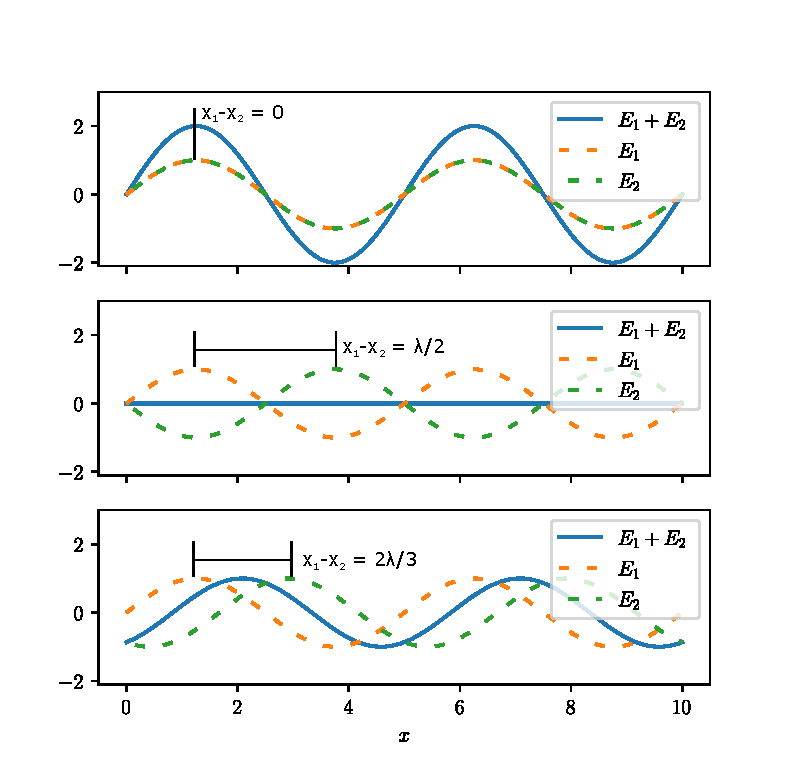
\includegraphics[width=0.5\linewidth]{Laserfysik/billeder/interferens.pdf}
    \caption{Interferens mellem elektromagnetiske bølger fra de to veje i et interferometer. I det øverste plot er der ingen vejlængdeforskel, og det totale E-felt viser \emph{konstruktiv interferens}. I det midterste plot er vejlængdeforskellen lig med bølgelængden af lyset, og der er \emph{destruktiv interferens}. Det nederste plot er et sted der imellem, der viser let destruktiv interferens.}
    \label{laser:fig:interferens}
\end{figure}

Vi kan komme nærmere ind på interferensen, ved at udregne den gennemsnitlige intensitet af denne kombinerede bølge. Det kræver, at vi sætter udtrykket herover i anden, og integrerer det fra $0$ til $2\cdot \pi$. Det tager lidt tid at løse, og metoden giver ikke nogen yderligere indsigt i det fysiske system, så derfor springer vi direkte til resultatet:
%
\begin{align}
    I_{avg} = \frac{c\cdot n \cdot \epsilon_0}{2}\frac{E_0^2}{4} \cdot \left( \cos\left({\frac{2\cdot\pi\cdot c}{\lambda}}(x_1-x_2)\right) + 1 \right)
\end{align}
%
Her ser vi, at intensiteten bliver 0, når cosinus bliver til $-1$, og bliver størst når cosinus er $+1$. Cosinus er $+1$, når det der står inde i den er 0, og bliver det igen, når det er $2\cdot \pi$. Man siger i så fald at argumentet til cosinus er henholdsvis $0$ eller $2\cdot\pi$. 
%
\begin{align}
    {\frac{2\cdot\pi}{\lambda}}(x_1-x_2) = 0 \implies x_1 - x_2 = 0\\
    {\frac{2\cdot\pi}{\lambda}}(x_1-x_2) = 2\cdot \pi \implies x_1 - x_2 = \lambda
\end{align}
%
Og det kan vi relatere til længden af armene i interferometeret, $s_1$ og $s_2$. ved hjælp af \cref{laser:eq:vejlangde}:
%
\begin{align}
    x_1 - x_2 = (2\cdot s_1 + l) - (2\cdot s_2 + l) = 2\cdot(s_1 - s_2).
\end{align}
%
Her kan vi altså se, at hvis vi varierer den relative vejlængde imellem de to arme med halvdelen af bølgelængden af lyset, så vil lyset gå hele vejen fra maximum til ingenting og tilbage til maximum igen. Dermed tillader interferometeret os at måle afstande helt ned til det halve af lysets bølgelængde meget præcist. I tilfældet af den Helium-Neonlaser, som vi skal bruge, er det helt ned til \SI{316.5}{\nano\meter}! Det eksperiment, der for nogle år siden målte tyngdebølger for første gang, er faktisk baseret på netop sådan et interferometer, fordi de havde brug for at måle meget små afstande.

\section{I virkeligheden}
I analysen af interferometret, har vi antaget at lysets elektriske felt er endimmensionelt. I øvelsen kommer vi til at se, at resultatet passer godt for midten af den rekombinerede lystråle på skærmen. I den virkelige opstilling vil lyset danne frynser, der bevæger sig når vejlængden varieres. Se \cref{laser:fig:frynser}. Figuren viser, at den perfekte opstilling har runde frynser, mens den lidt mindre perfekte opstilling har lige frynser. Dog er begge opstillinger fint brugbare i forhold til eksperimentet.

\begin{figure}
    \centering
    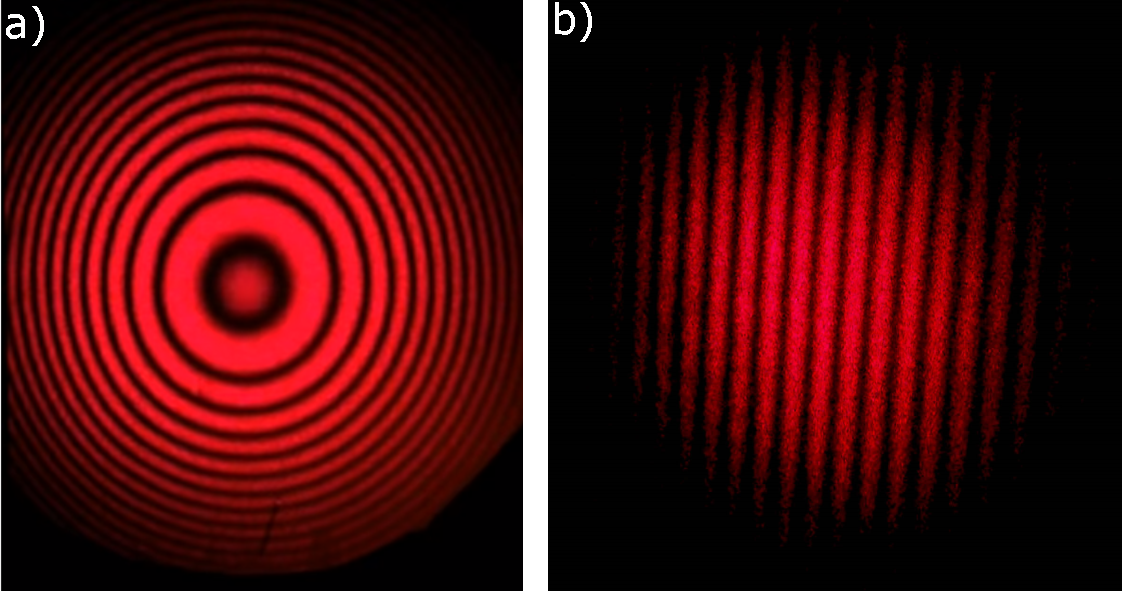
\includegraphics[width=0.45\linewidth]{Laserfysik/billeder/InterferenceFringes.pdf}
    \caption{Interferensfrynser i et Michelson-interferometer. a) runde frynser fra et perfekt opsat interferometer, hvor strålerne til sidst løber helt parallelt med hinanden uden forskydning. b) er ikke helt så godt sat op, og de lige frynser betyder, at strålerne ikke løber helt parallelt med hinanden.}
    \label{laser:fig:frynser}
\end{figure}


\nocite{griffithsIntroductionElectrodynamics2018}

\end{document}